%TODO Spustit program vlna


% Vlozi hlavicku s nastavenim a obecnymi balicky
\documentclass[11pt,a4paper,onecolumn,notitlepage]{article}
\usepackage[czech]{babel}
\usepackage[utf8]{inputenc}
\usepackage{lmodern}
\usepackage[T1]{fontenc}
\usepackage[text={17cm, 24cm},left=2cm,top=3cm]{geometry}
\usepackage{graphicx}
\usepackage{enumitem}
\usepackage[bottom]{footmisc}
\usepackage{xstring}

\usepackage{float}

\floatstyle{plain}
\newfloat{plaintext}{htp}{lop}

\usepackage{xfrac}

\usepackage{color}
\usepackage[unicode,colorlinks,hyperindex,plainpages=false,pdftex]{hyperref}
\usepackage[all]{hypcap}

\graphicspath{ {./img/} }


\providecommand{\todo}[1]{\section{[TODO] #1}}


% Jméno předmětu
\newcommand\courseShortcut{GMU}
\newcommand\courseName{Grafické a multimediální procesory}
\newcommand\projectName{Příprava na zkoušku}



\begin{document}
	
\includegraphics{FIT.pdf}

\begin{center}
	\vspace{\stretch{0.382}}
	\LARGE
	\courseName\ (\courseShortcut)\\
	\Huge
		\projectName\\
	\vspace{\stretch{0.618}}
	\normalsize
	\url{https://github.com/VasaMM/GMU-otazky}
	\hfill
	\today
\end{center}


\pagenumbering{gobble}


\newpage
\pagenumbering{arabic}
\tableofcontents
\newpage




\section{Popište základní principy návrhu energeticky úsporného procesoru CPU/GPU, jak se vyhodnocuje energetická úspornost.}
	\todo


\section{Popište vývoj 2D/3D grafického řetězce s různým stupněm zřetězení.}
	\begin{figure}[h]
		\centering
		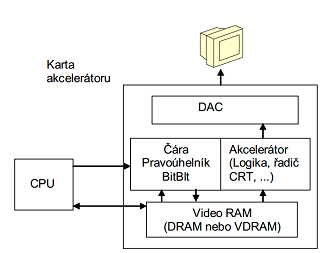
\includegraphics[width=0.6\textwidth]{ZakladniKarta.png}
		\caption{Základní 2D zpracování (IBM 8514)}
		\label{fig:ZakladniKarta}
	\end{figure}

	\begin{figure}[h!]
		\centering
		\includegraphics[width=0.8\textwidth]{ackey.png}
		\caption{Akeleyho pipeline}
		\label{fig:ackey}
	\end{figure}
	generovanie $\rightarrow$ traverzacia $\rightarrow$ transformacia $\rightarrow$ rasterizadia $\rightarrow$ zobrazenie (display) Implementovana napr. u i740, Savage3D


\section{Popište 1- až n-rozměrné multiprocesorové propojovací struktury (Origin/Onyx) a typy propojovacích sběrnic Silicon Graphics.}
	\subsection*{Origin}
		Propojovací struktura architektury koncepce Origin2000 umožnuje vytváret až 5D krychle. Díky její pružnosti a koncepcní pokrokovosti byla prevzata i do navazujících architektur SGI, jako napríklad Onyx2, a další.
		
		Architektura Origin2000 je tvorena množstvím výpoctových uzlu, propojených navzájem propojovací sítí CrayLink. Každý výpoctový uzel obsahuje jeden nebo dva procesory s pametí cache, sdílenou pamet, adresár pro rízení koherence cache s hlavní pametí a dve ruzné jednotky interface – jeden, XIO, který pripojuje I/O jednotky, a druhý, CrayLink, propojující uzly pres jednotku Router.

	\subsection*{Onyx2}
		Každý procesor je spolu se svou pamětí cache a částí operační paměti počítače (o kapacitě od 128 MB do 8 GB) součástí jednoho procesorového uzlu, který obsahuje čtyři procesory. Obousměrný přenos dat mezi procesory v jednom uzlu dosahuje hodnoty 1,6 GBs-1, resp. 800 MBs-1 v každém směru zvlášť. Jednotlivé uzly jsou mezi sebou propojeny pomocí propojovací sítě, jejíž topologie sice vychází z ideální hyperkrychle, ale z důvodu optimalizace datových přenosů jsou mezi uzly vytvořeny i další přídavné datové spoje (již z principu musí jít o diagonály), zejména mezi procesory a zobrazovacími subsystémy.
	

\section{Popište principy výstavby, činnosti a použití GPGPU.}
	Jde o techniku využití GPU k obecným (negrafickým) výpočtům, které běžně probíhají na CPU. Zatímco dříve bylo zpracování dat na GPU pevně dané (static pipeline), dnes už je převážná část programovatelná, a tudíž nabízí možnost obecných výpočtů. K tomu slouží např. rozhraní OpenCL, CUDA či ATI Stream.
	
	Z povahy grafických čipů vychází také způsob práce s daty, který je silně orientován na paralelní proudové zpracování dat. Data jsou často rozdělena do 2D mřížky, kde nad každou buňkou pracuje jedna výpočetní jednotka. Tyto jednotky sdílí kód programu, nazývaný také kernel. Možnost synchronizace či sdílení dat mezi jednotkami v průběhu výpočtu je omezená a značně snižuje výsledný výkon. (Alespoň v OpenCL možnost sdílení paměti existuje.) Z běžných součástí GPU lze použít například texturovací jednotky jako vstupní rozhraní a framebuffer jako výstupní.
	
	Syntaxe programovacího jazyka může být podmnožinou jazyka C (v OpenCL), ovšem existují omezení plynoucí právě z paralelního proudového zpracování. Není možné používat rekurzi, volání vnořených funkcí má svá omezení, jsou zavedeny speciální funkce a datové typy pro práci s vektory, je žádoucí znovuvyužívat použité proměnné a obecně musí optimalizace probíhat jinak než u běžných (CPU) programů - s ohledem na povahu HW.
	
	Vhodnými úlohami pro zpracování na GPU je například zpracování videa, zvuku či řeči, provádění fyzikálních simulací (kapaliny, osvětlení, počasí) anebo třeba úlohy z kryptografie.


\section{Popište koncepci a vlastnosti různých typů Streaming Multiprocesoru}
	\todo
	
	
\section{Popište principy komprese dat v systému Pascal (delta-komprese a další).}
	\todo
	
	
\section{Popište architekturu grafických multiprocesorů a nové principy činnosti, jako komprese dat, preempce a její typy.}
	\todo
	
	
\section{Popište princip tensorového jádra Turing, k čemu slouží, jaké formáty dat se používají.}
	\todo


\section{Popište principy a funkce preempce Pascal.}
	\todo
	
	
\section{Popište vývoj unifikovaného adresového prostoru, principy činnosti, a jeho hardwarovou podporu.}
	\todo
	
	
\section{Popište principy návrhu energeticky úsporného GPU pro mobilní zařízení.}
	\todo
	
	
\section{Popište hlavní vývojové etapy a principy grafických systémů Mali pro mobilní zařízení.}
	\todo
	
	
\section{Vysvětlete a zdůvodněte koncepci kachliček (tiles) 16x16 pixelů v grafice Mali.}
	\todo
	
	
\section{Popište formáty dat podporované v grafice Mali, skalární i vektorové.}
	\todo
	
	
\section{Popište a zdůvodněte principy tří základních typů komprese textur - ztrátové, bezeztrátové a adaptivní.}
	\todo
	
	
\section{Popište alespoň 3 rozdíly mezi architekturami GPU a CPU.}
	\todo
	

\section{Co je to kernel?}
	\todo


\section{Co je to vlákno?}
	\todo


\section{Co je to divergence vláken a kdy vzniká?}
	\todo


\section{Co je to warp/wavefront?}
	\todo


\section{Co je to multiprocesor (streaming multiprocessor/compute unit) GPU a k čemu slouží.}
	\todo


\section{Co je to fronta příkazů (command queue)?}
	\todo


\section{Jakým způsobem je možné synchronizovat úlohy ve frontě příkazů s vykonáváním mimo pořadí (out-of-order execution) nebo mezi frontami v OpenCL?}
	\todo


\section{Jakým způsobem se eliminuje/zmírňuje dopad aritmetických/paměťových latencí.}
	\todo


\section{Co je to konflikt banků v lokální paměti a kdy vzniká?}
	\todo


\section{Co je to zarovnaný přístup do paměti?}
	\todo


\section{Popište konstantní/uniformní paměť.}
	\todo


\section{Popište lokální/sdílenou paměť.}
	\todo


\section{K čemu slouží texturovací jednotky?}
	\todo


\section{Jaké jsou rozdíly mezi bufferem a texturou v OpenCL?}
	\todo


\section{Jaký je rozdíl mezi normalizovanými a nenormalizovanými texturovacími koordináty?}
	\todo


\section{Co je to register spilling?}
	\todo


\section{Jaké jsou způsoby komunikace mezi vlákny ve skupině a mezi skupinami?}
	\todo


\section{K čemu slouží atomické instrukce? Popište jejich vlastnosti a příklad algoritmu kde je možné je využít.}
	\todo


\section{Jaké mohou být příčiny nízké výkonnosti kernelů?}
	\todo


\section{Co je to obsazenost multiprocesoru (occupancy), na čem je závislá?}
	\todo


\section{Co je to aritmetická a paměťová latence?}
	\todo


\section{Co je to separabilní filtr a jakým způsobem lze přistupovat k jeho paralelizaci?}
	\todo


\section{K čemu slouží paralelní redukce?}
	\todo


\section{Co je to dynamický paralelismus?}
	\todo


\section{Jaké jsou možné typy přenosů dat mezi CPU a GPU?}
	\todo


\section{K čemu slouží P2P přístup a jakým způsobem ho lze využít.}
	\todo


\section{K čemu slouží operace shuffle?}
	\todo


\section{Vyjmenujte alespoň 3 api pro GP-GPU.}
	\todo


\section{Co to je SpirV?}
	\todo


\section{K čemu slouží operace ballot?}
	\todo


\section{K čemu lze využít atomicCompSwap?}
	\todo


\section{Jaký je vztah mezi NDRange/Grid/Dispatch, pracovní skupinou a vláknem/invokací?}
	\todo


\section{Jaké paměti jsou na GPU a popište jejich vlastnosti (odkud je lze plnit, odkud je lze číst, relativní rychlost, relativní velikost).}
	\todo


\section{Jaký je rozdíl mezi pracovní skupinou a warpem/wavefrontem.}
	\todo


\section{K čemu slouží příkaz barrier? Jakou má souvislost s rozdělením vláken do skupin, warpů? Jaký to má vztah k větvení programu?}
	\todo


	
\end{document}          
